% !TEX root = ../main.tex
\subsection*{Schools of Magic} \label{ssec::schoolsofmagic}
% TODO. The whole magic system is being updated. See to it that this subsection reflects that.

\subsubsection{Bonereading\\ \small{Mevthan}}
Long before Tanethism became the official religion of Khedrat, the art of bonereading was already a common practice among its populace.
By using the bones of marine creatures as catalysts, witch doctors of antique were able to listen to the wisdom of their divinities.
After hearing the plights of the common gats, the gods could influence events to help - or punish - those who deserved it, and witch doctors were of high regard in society thanks to this ability.

As the art developed over time, new spells and incantations have appeared.
The bones are now used for more than divination, but as ways to directly influence the reader's surroundings in more direct manners.
Nowadays, bonereading remains an important part of Khedrat's culture, and is still practiced both by the farmer to ask for a good harvest, by the sailor to attain a safe voyage, and by priests exert the gods' will.

% Some maintain the argument that bonereading is not a form of communication with the gods, but that the magic lies in the bones themselves.
% Such words fall on deaf ears in the common gat, and are considered heresy by the church, punishable by exile.

\begin{table*}[b]%
    \begin{DndTable}[width=\linewidth]{X}
        \centering
        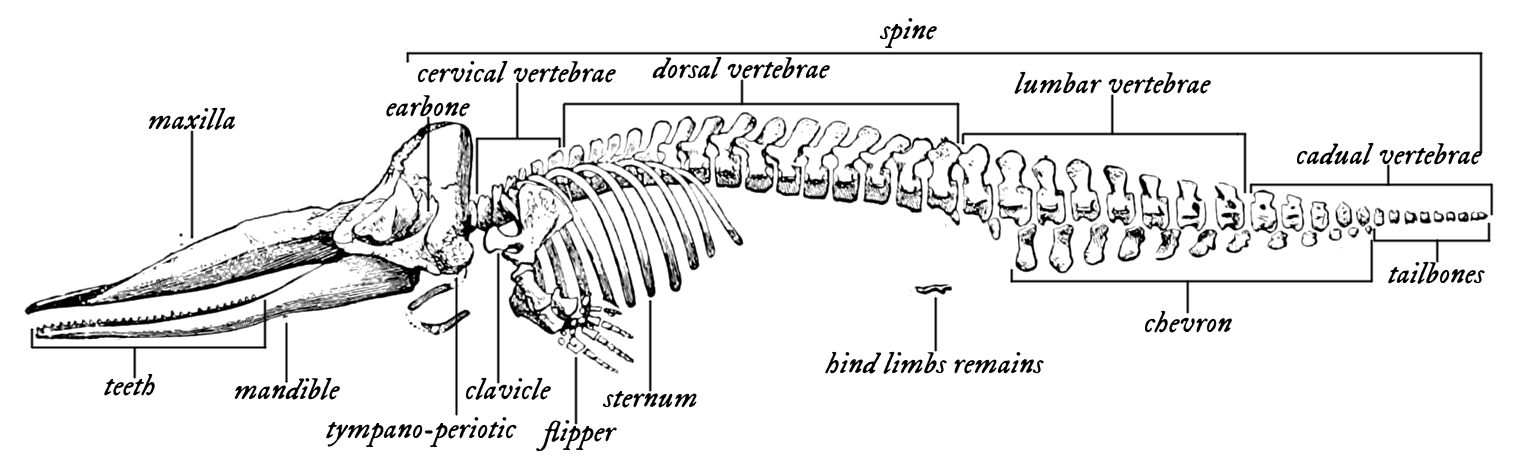
\includegraphics[width=0.99\textwidth]{01yuadrem/img/23sperm_whale_skeleton.png}
    \end{DndTable}
\end{table*}

\subsubsection{Wordbinding\\ \small{Dremshamad}}
Well known is the obsession of the many houses of Palegna with words, names, and languages, and evidence of this is wordbinding.
Wordbinding, or Dremshamad in dust tongue, is the art of giving strength to words so that, no matter the medium, their mere utterance conveys an tangible effect in the world.
Its spells are many and varied, like saving effects in scrolls or books to be invoked later, binding the will of creatures by using their true names, and speaking command words that can't be disobeyed by any mean.

Perhaps the most meaningful product of wordbinding are reflexive contracts.
These agreements bind through the strength of words alone, enforcing their terms upon the signing parties by tying harsh effects to the rights and duties specified.
Always produced in triplicate with each requiring three signatures per party, reflexive contracts are practically unvoidable, thus regarded as the perfect mean to ensure cooperation between beings, houses, or even entire nations.

% Crafting a document with words of power:
% * List of effects that can be produced (more are unlocked as expertise increases)
% * Interaction with words that produce such effect (spoken out loud, whispered, listened to, read)

% All contracts must have a clause that can void the contract by design. Most usually it is being burned by the fire of a wyrm, since this act is neigh impossible without dying.

\subsubsection{Windherding\\ \small{Dentrala}}
Perilous are the winds from the southern ocean, relentlessly tearing apart any ship that dares sail it's turbulent waters.
Many forget that the many tribes from the Qul archipelago had to deal with these strong winds and storms in their daily lives.
To face this, they slowly developed a complex system of sympathetic magic.

By standing atop large poles within eyesight of each other, ird witches from the dentralin tribe managed to stop the wind simply by holding their breath.
This practice gave rise to a wide array of wind-based spells that the tribe wise to use to their advantage during the tunsal wars, and eventually led to the establishing of Jenkash.

\subsubsection{Sigaldry\\ \small{Guen Tsue}}
Unlike other languages, the naenk tongue is deeply rooted in nature itself, and can be used to even directly talk to it, with seedspeech being the clear example.
This quality of the language led to Gannag's shamans to develop a writing system that can evoke effects when interacted with, called shinerunes.

The tsaneks of Gannag use this method to create self-triggering traps, which are set about villages to catch prey and ward off would-be invaders.
Apart from this, intricate shinerunes are used to many different effects, such as a silent bell alerting of the presence of a stranger in a dwelling, a self-heating plate to boil water in, or clothes that spontaneously heat up as a reaction to bad weather.
Truly, the capabilities of shinerunes are only limited by the creativity and skill of their author.

\begin{table*}[t]%
    \begin{DndTable}[width=\linewidth, header=\centering Knaenese Alphabet]{X}
        \centering
        
\includegraphics[width=0.99\textwidth]{01yuadrem/img/23knaenese_sample.png}
    \end{DndTable}
\end{table*}

\subsubsection{Psionics} % NOTE. I don't like the name but it's not that bad I guess.
Perhaps the strangest part of the zaloths is the fact that they do not speak through a mouth, but directly into other beings' minds.
This ability is only made possible by the special nature of the zaloths themselves, and is very rarely seen in the other kins, in peculiar gifted individuals.
Not limited to telepathy however, the art developed into a plethora of mind-based abilities known as psionics.

Psionics are fueled by one's own mind without external sources of energy, meaning that the art exerts a great effort from the author.
The zaloths have elaborated varied psionic effects to date, expanding their original telepathy to more tangible effects, like clairvoyance, telepathy, and many mind-altering effects.

\subsubsection{Similarity Sympathy}
% Blink (quantum teleport): Cantrip to teleport, only usable if being perceived by no sentient being when moving to an area not perceived by any sentient being. Hard to use in most cases yet extremely powerful in certain scenarios. (Mechanically it's a cantrip but using it is actually tiring, so it can't really be used as a reliable method of transportation).
% The best thaumaturges are blind FUCK YES!!

No one can deny that Yuadrem completely changed after the schism.
The ash storm ravaged the land and caused the 9 year famine, tens of thousands of strange creatures poured in, and new, alien kins settled into the land.
For better or for worse, the event transformed the fabric of reality.
Soon after the schism the witches and shamans of the early world started to experiment with a new and strange form of magic: the Similarity Link.

This link is a strange form of sorcery which seems to follow different rules than the other schools.
It affects directly the physical properties of objects and creatures, like making rocks weight as little as feathers, or changing the size of other creatures.
Perhaps the strangest part of this is that it seems to behave differently depending on if it's being perceived or not.%, and thaumaturges take advantage of this by covering their eyes when casting certain spells.

\subsubsection{Tidal Manipulation\\ \small{Rashid}} % !!
Rashid involves manipulating the tides in the air or in others to attain one's goals.
Originally taught by the sole survivor of the Rashiist school of thought, it ranges from simple charms and illusions to potent spells with effects that vary depending on the caster's or target's tidal alignment.

Every Rashid user knows that they must exercise their magic in secrecy, since the practice is severely punished due to Rashiism's dark history.
The most experienced in the art however know that the one they truly have to fear is the Sorrow.
The Sorrow is the being that destroyed the Rashiist school of thought, leaving the pale blemish as a warning to any who dares follow their teachings.

\subsubsection{Fleshshaping\\ \small{Cthai'khas}} % !!
Recently reborn in the breathing city of Cabb Goem-Rlamesh is the almost lost art of Ukarilth: fleshshaping.
An everyday act of the tall kin, fleshshaping is a kind of magic that involves transfiguring the flesh of the caster or of others nearby, be them alive or dead.

While most fleshshapers remain in their putrid island, some have started to show up in the eastern parts of Yuadrem, and the art is slowly being spread by concealed mages.
A strange attribute of fleshshaping that sets it apart from the other schools is that its effect vary depending on the species of the caster.
For example, while a gat can mold its flesh to temporarily use its bones as weapons, a naenk can grow roots into the floor to catch prey, and a quies can reinforce its wooden exterior in preparation for an attack.
